	\documentclass{article}
			
		\usepackage{parskip}
		\usepackage{listings}
		\usepackage{xcolor}
		\usepackage{textcomp}
			
		%STYLE AND COLOR DEFINITION FOR SOURCE CODE 	
		\newcommand{\PHPamountofcolor}{75}
		\newcommand{\SourceCodeContext}{5}
		%Lets define the php language colors:
		\definecolor{PHP_comment_old}{HTML}{FF8000}
		\colorlet{PHP_comment}{PHP_comment_old!\PHPamountofcolor!black}
		\definecolor{PHP_default_old}{HTML}{000000}
		\colorlet{PHP_default}{PHP_default_old!\PHPamountofcolor!black}
		\definecolor{PHP_keyword_old}{HTML}{6c9c11}
		\colorlet{PHP_keyword}{PHP_keyword_old!\PHPamountofcolor!black}
		\definecolor{PHP_emph1_old}{HTML}{0F58A2}
		\colorlet{PHP_emph1}{PHP_emph1_old!\PHPamountofcolor!black}
		\definecolor{PHP_emph2_old}{HTML}{CCAA00}
		\colorlet{PHP_emph2}{PHP_emph2_old!\PHPamountofcolor!black}
		\definecolor{PHP_emph4_old}{HTML}{C60484}
		\colorlet{PHP_emph4}{PHP_emph4_old!\PHPamountofcolor!black}
		\definecolor{PHP_string_old}{HTML}{C78F0A}
		\colorlet{PHP_string}{PHP_string_old!\PHPamountofcolor!black}
		\definecolor{PHP_variable_old}{HTML}{C82210}%C82210
		\colorlet{PHP_variable}{PHP_variable_old!\PHPamountofcolor!black}
		\definecolor{PHP_number_old}{HTML}{BF1CA6}
		\colorlet{PHP_number}{PHP_number_old!\PHPamountofcolor!black}
		%Now we want to highlight the variables. This will be done by triggering the function \PHPhighlightvar at the start of any $ run. This function wil only highlight variables and any other identifiers will be ignored. Luckily lstlisting will only give correct identifiers so we only will have to check if the previous call was made with a $
		\usepackage{fontspec}
		\setmonofont{Courier}
		%\usepackage[utf8]{inputenc}
		%\usepackage[T1]{fontenc}
		%\usepackage{courier, textcomp}
		\usepackage{etoolbox}
		\newtoggle{InString}{}% Keep track of if we are within a string
		\togglefalse{InString}% Assume not initally in string
		
		\newcommand*{\ColorIfNotInString}[1]{\iftoggle{InString}{#1}{\color{PHP_number}#1}}%

		%helper
		
		\newcommand{\PHPhighlightvar}[1]{\ifnum\theDollarFlag=1 \color{PHP_variable} \fi#1\setcounter{DollarFlag}{0}}
		\newcounter{DollarFlag}
		
		%images
		\usepackage{graphicx}
		\graphicspath{ {images/} }
		\usepackage{wrapfig}
		\usepackage{subcaption}
		
		
			
			
			
		
			
			\title{Machine Learning: Second Home Work \\ \bigskip \large  Polynomial Regression}

			\author{Edoardo Ghini}
			
			\begin{document}
			
			\textbf{\maketitle}
			\pagenumbering{gobble}
			
			\bigskip\bigskip\bigskip
			\begin{center}
			
\includegraphics[width=0.5\textwidth]{laSapienza}
			\end{center}
			\bigskip\bigskip\bigskip
			\textbf{
			Dipartimento di Ingegneria dell'Università di Roma La Sapienza}
			

			\newpage
			\pagenumbering{roman}
			\tableofcontents
			\newpage
			\pagenumbering{arabic}
			
			
			
			
			
			%SETTING STYLE OF SOURCE CODE
			\lstset{
		  language        = php,
		  basicstyle      = \footnotesize\ttfamily,
		  keywordstyle    = \color{PHP_keyword},
		  stringstyle     = \color{PHP_string!90!black}\toggletrue{InString},
		  %this allows highlighting of variables:
		  literate        =  {\$}{{\iftoggle{InString}{\$}{\setcounter{DollarFlag}{1}\color{PHP_variable}\$\color{PHP_default}}}}1
		%    {"}{{{\ProcessQuote{"}}}}1% Disable coloring within double quotes
		%    {'}{{{\ProcessQuote{'}}}}1% Disable coloring within single quote
		    {0}{{{\ColorIfNotInString{0}}}}1
		    {1}{{{\ColorIfNotInString{1}}}}1
		    {2}{{{\ColorIfNotInString{2}}}}1
		    {3}{{{\ColorIfNotInString{3}}}}1
		    {4}{{{\ColorIfNotInString{4}}}}1
		    {5}{{{\ColorIfNotInString{5}}}}1
		    {6}{{{\ColorIfNotInString{6}}}}1
		    {7}{{{\ColorIfNotInString{7}}}}1
		    {8}{{{\ColorIfNotInString{8}}}}1
		    {9}{{{\ColorIfNotInString{9}}}}1,
		  identifierstyle = \color{PHP_default}\PHPhighlightvar,
		  commentstyle    = \color{PHP_comment}\slshape,
		  emph            =[1]{require_once, require, include_once, include, namespace, use, class, function, new},
		  emphstyle       =[1]\color{PHP_emph1},%\bf,
		  emph            =[2]{echo, empty, isset, array, instanceof},
		  emphstyle       =[2]\color{PHP_emph2},%\bf,
		  emph            =[3]{var, const, abstract, 
		                        protected, private, public,
		                        static, final, extends, implements,
		                        global, if, else, foreach ,for,
		                        endforeach, endif, endfor, elseif,
		                        as},
		  emphstyle       =[3]\color{PHP_keyword},%\bf,
		  emph            =[4]{return, throw, exit, __halt_compiler, continue, break},
		  emphstyle       =[4]\color{PHP_emph4},%\bf,
		  breaklines      = true,
		  captionpos      = b,
		  rulecolor       =\color{black},
		  keywords    ={__halt_compiler,    abstract,   and,    array,
		                    as, break,  callable,   case,   catch,  class,
		                    clone,  const,  continue,   declare,    default,
		                    die,    do, echo,   else,   elseif,
		                    empty,  enddeclare, endfor, endforeach, endif,
		                    endswitch,  endwhile,   eval,   exit,   extends,
		                    final,  finally,    for,    foreach,    function,
		                    global, goto, if,   implements, include,
		                    include_once,   instanceof, insteadof,
		                    interface,  isset, list,    namespace,
		                    new,    or, print, private, protected,  public,
		                    require,    require_once, return,   static,
		                    switch, throw,  trait, try, unset, use, var,
		                    while,  xor,    yield,
		  },
		  numbers=left,
		  stepnumber=1,  
		  numberfirstline=true,
		  numberstyle=\footnotesize,
		  xleftmargin=4.0ex,
		  upquote=true,
		  showlines=true
		  }	
			
			\renewcommand{\lstlistingname}{Code}

			
			\part{Introduction}
			
				\section{Scope}
This experience should bring to light the inadequacy of a linear approach when we are treating a non linear distribution of data points.
				\section{Objectives}
				It would be required to train a non-linear model with a simple polynomial expansion approach that allows to achieve regression of the dataset in fig(1), chasing a minimum value of the mean square error. 
				\begin{center}
\begin{figure}
\centering
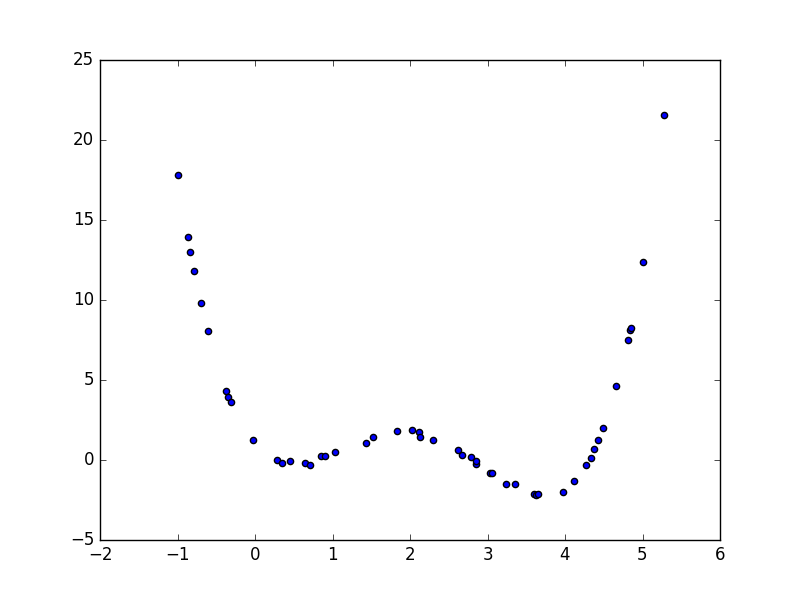
\includegraphics[width=0.9\textwidth]{data-plot}
\caption{}
\label{fig:1}
\end{figure}
\end{center}

\newpage
			\part{Development}
				\section{Data loading}
	At  the beginning , the dataset was loaded, it was already divided in training and test sub-sets and in input values and corresponding labels.
	Then I standardised the input sub-sets and so, done that, I was ready to approach the training phase.
	
	
	

				\section{Training}
				
				
				\subsection{Linear Model}
				In order to show the inadequacy of a linear approach I trained a linear regressor with input data and I plotted the result,  as shown in fig(2).
				\begin{center}
\begin{figure}
\centering
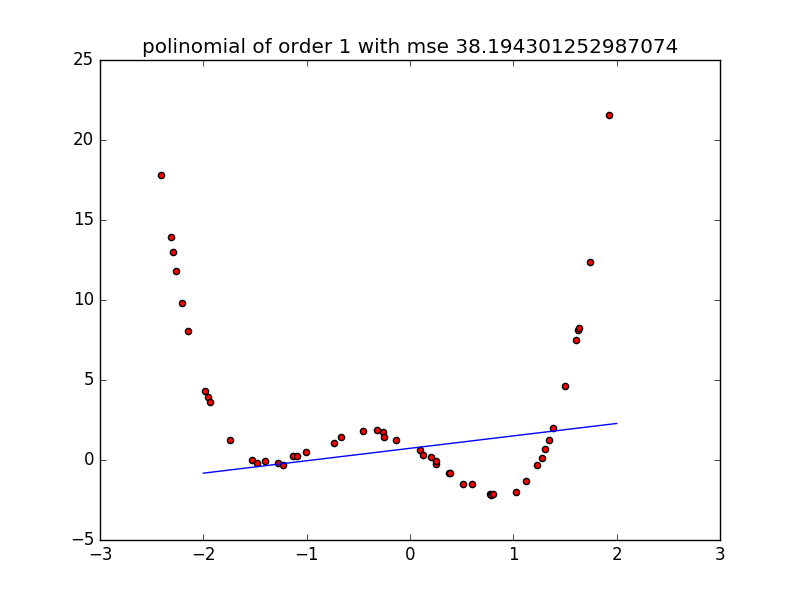
\includegraphics[width=0.9\textwidth]{poli-order-1}
\caption{}
\label{fig:2}
\end{figure}
\end{center}
				\subsection{Polynomial Model}
				Subsequently I applied a polynomial expansion to input data, that consists in adding terms that are computed by a an exponentiation of the single input terms to obtain a polynomial of higher grade than the beginning.
				Above, there are some polynomial expansions that I considered in order to find the order that best fits the actual dataset.
				
\begin{figure}
\centering
        \begin{subfigure}[b]{0.48\textwidth}
                \centering
                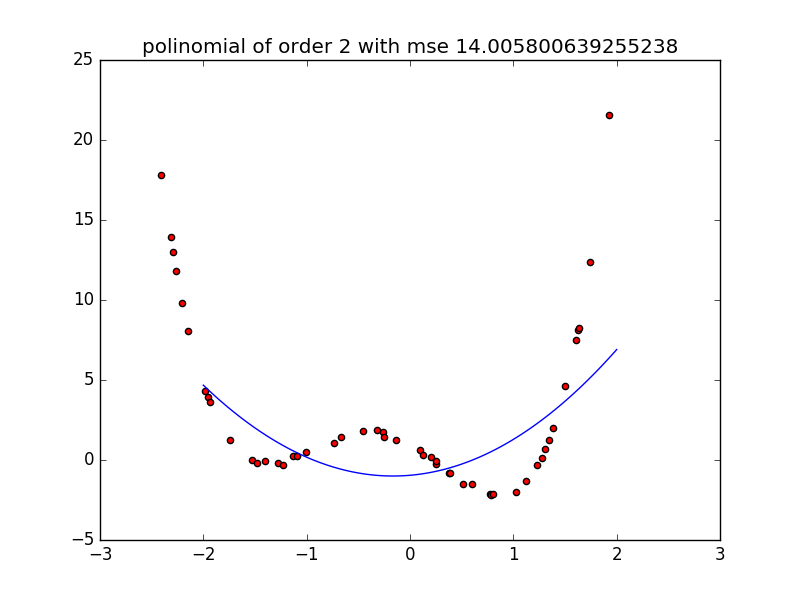
\includegraphics[width=\linewidth]{poli-order-2}
        \end{subfigure}\hfill
        \begin{subfigure}[b]{0.48\textwidth}
                \centering
                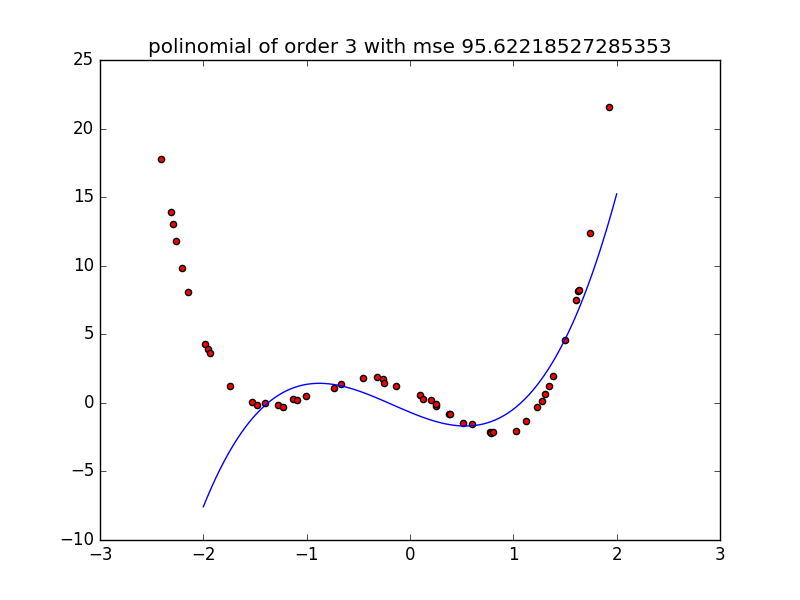
\includegraphics[width=\linewidth]{poli-order-3}
        \end{subfigure}\hfill
 \label{fig:3}
 \end{figure}
       
\begin{figure}
\centering  
        \begin{subfigure}[b]{0.48\textwidth}
                \centering
                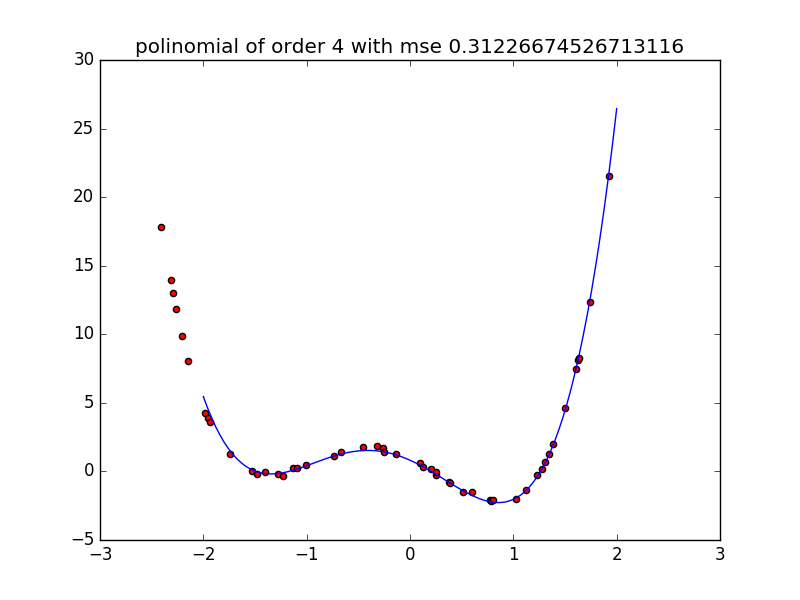
\includegraphics[width=\linewidth]{poli-order-4}
        \end{subfigure}\hfill
        \begin{subfigure}[b]{0.48\textwidth}
                \centering
                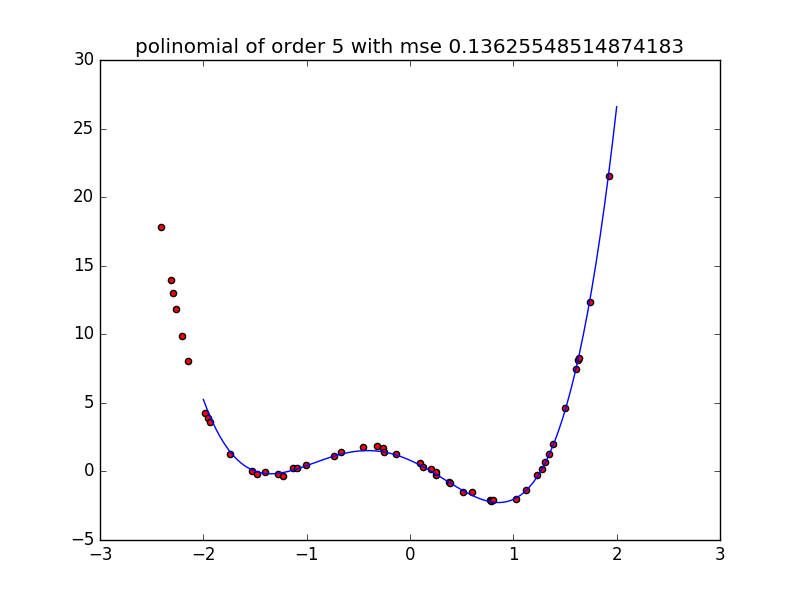
\includegraphics[width=\linewidth]{poli-order-5}
        \end{subfigure}
        \label{fig:4}
\end{figure}

\begin{figure}
\centering
        \begin{subfigure}[b]{0.48\textwidth}
                \centering
                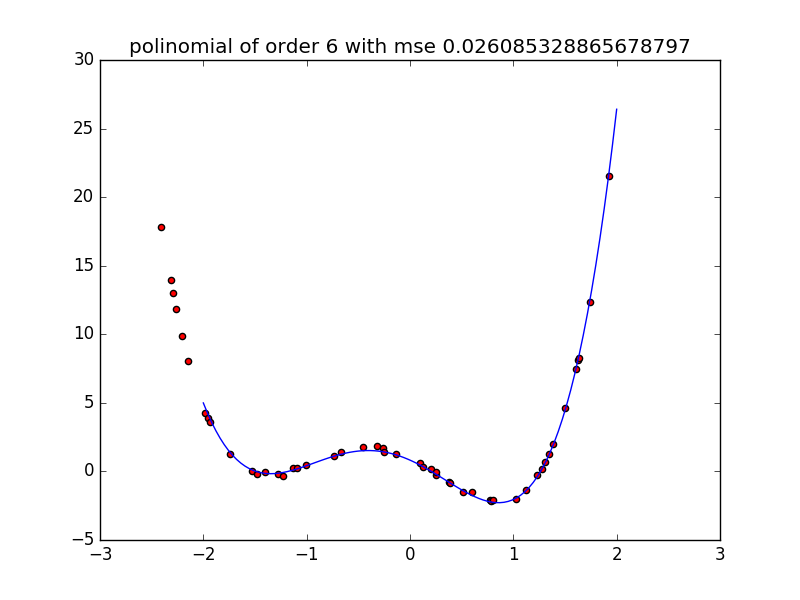
\includegraphics[width=\linewidth]{poli-order-6}
        \end{subfigure}\hfill
        \begin{subfigure}[b]{0.48\textwidth}
                \centering
                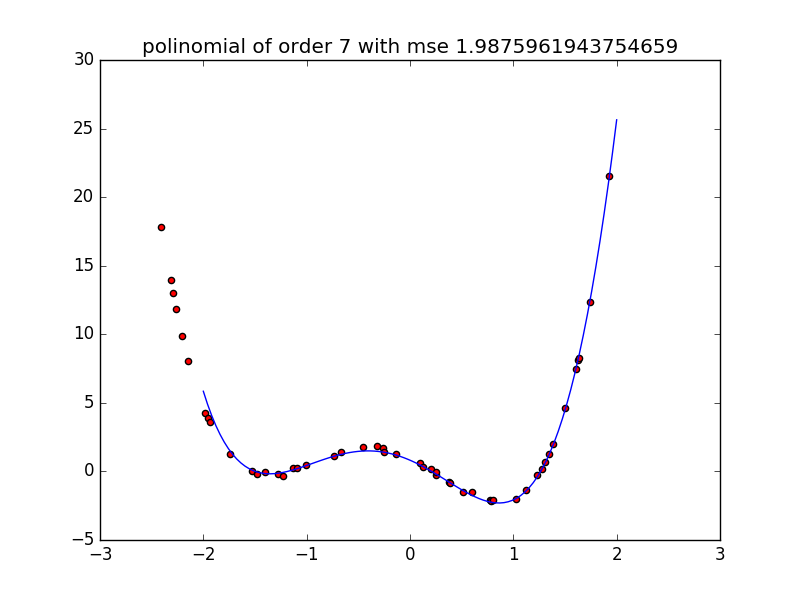
\includegraphics[width=\linewidth]{poli-order-7}
        \end{subfigure}\hfill
        \label{fig:5}
 \end{figure}
       
\begin{figure}
\centering  
        \begin{subfigure}[b]{0.48\textwidth}
                \centering
                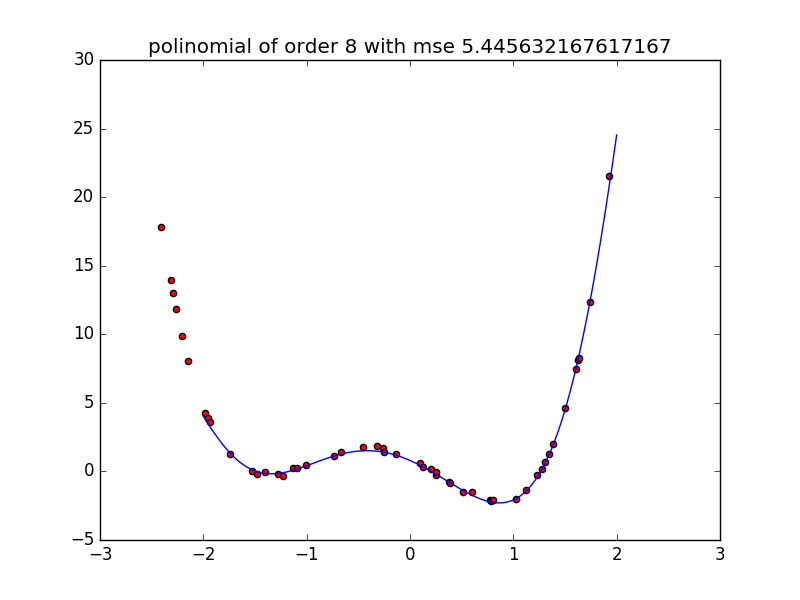
\includegraphics[width=\linewidth]{poli-order-8}
        \end{subfigure}\hfill
        \begin{subfigure}[b]{0.48\textwidth}
                \centering
                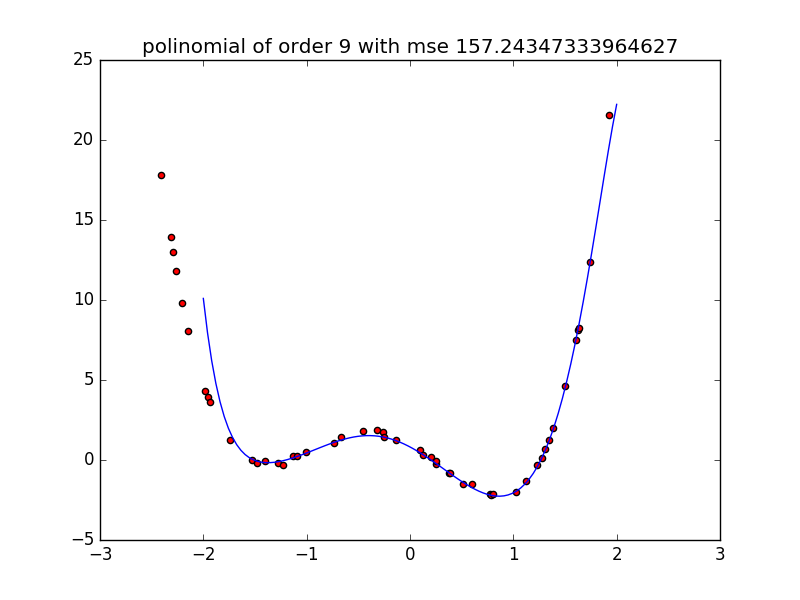
\includegraphics[width=\linewidth]{poli-order-9}
        \end{subfigure}
        \label{fig:6}
\end{figure}


				\subsection{Error Minimization}
				During the various polynomial grade incrementing iteration I kept track of the mean square error value brought from each polynomial and it turned out that the sixth grade polynomial was the best performer in the regression task.
				In fig(11) I have represented the mean square error function with the respect of the variation of the grade of the polynomial.
									\begin{center}
\begin{figure}
\centering
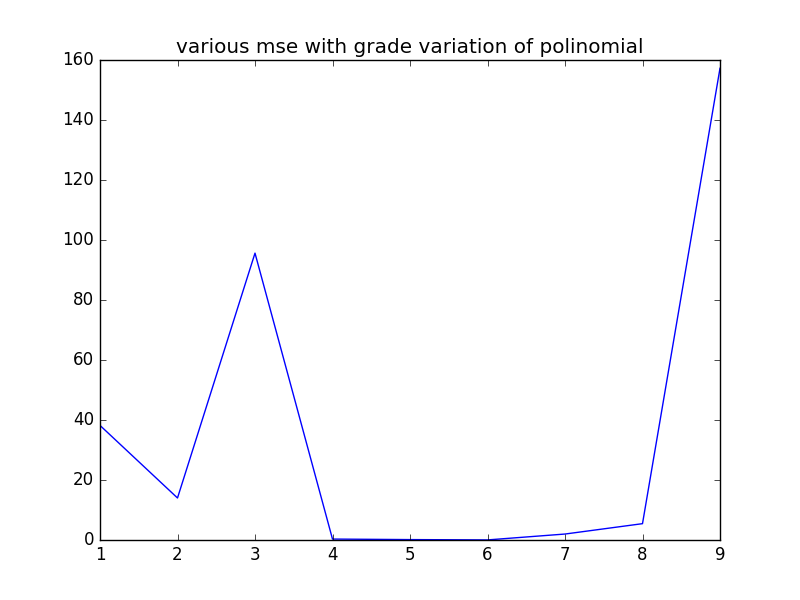
\includegraphics[width=0.9\textwidth]{grade-polivariation-mse}
\caption{}
\label{fig:7}
\end{figure}
\end{center}



\newpage
			\part{Conclusions}
				
			Finally, considering the collected results,  increasing the grade of the polynomial over the threshold, that for this dataset seems to be eight, causes a steep increment of the mean square error. This phenomenon is due to the overfitting of the model indeed. Under those circumstances the model will fit extremely well on the training data but on the other hand it will perform poorly on the test datas.
			
		\end{document}
